\setAuthor{Jaan Kalda}
\setRound{lõppvoor}
\setYear{2010}
\setNumber{G 9}
\setDifficulty{9}
\setTopic{Geomeetriline optika}

\prob{Punktallikad}
Juuresoleval joonisel on neli punkti, millest kaks on valgusallikad ja kaks nende tõelised kujutised, mille on tekitanud õhuke lääts. Leidke konstrueerimise teel läätse tasand ja optiline peatelg. Kui võimalusi on rohkem kui üks, siis leidke need kõik.

\begin{center}
	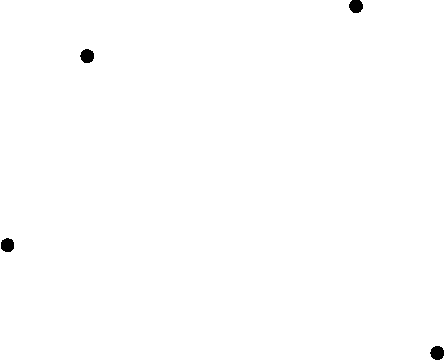
\includegraphics[width=0.3\linewidth]{2010-v3g-09-punktid}
\end{center}

\hint
Allikat ja kujutist ühendav sirge läheb läbi läätse keskpunkti, kusjuures läätse keskpunkt peab jääma allika ja kujutise vahele, sest tegu on tõelise kujutisega. Lisaks teame, et sirge kujutis on sirge, kusjuures need kaks sirget lõikuvad läätse tasandis.

\solu
Allikat ja kujutist ühendav sirge läheb läbi läätse keskpunkti ning see punkt peab jääma allika ja kujutise vahele, sest kujutis on tõeline.
Seetõttu saame läätse keskpunkti $O$ leida kui lõikude $S_1S_1^\prime$ ning $S_2S_2^\prime$ lõikepunkti, kus $S_1$ ja $S_2$ on allikad ning $S_1^\prime$ ja $S_2^\prime$
on vastavad kujutised. Et lõikepunkt tekiks, peavad $S_1$ ja $S_1^\prime$ paiknema diagonaalselt. Edasi paneme tähele, et sirge kujutis on sirge, kusjuures
need kaks sirget lõikuvad läätse tasandis. Et sirge $S_1S_2$ kujutis on $S_1^\prime S_2^\prime$, siis nende lõikepunkt $P$ võimaldab meil leida juba
läätse tasandi $OP$; optiline peatelg on punktist $O$ tõmmatud ristsirge Läätse tasandi seisukohast pole oluline, kumb sirgetest ($S_1S_2$ või $S_1^\prime S_2^\prime$) on kujutis ja kumb originaal.
Seetõttu tekib meil kaks oluliselt erinevat võimalust: kas need kaks sirged paiknevad ligikaudu horisontaalselt või ligikaudu vertikaalselt, vt joonist.\\

\begin{center}
	\includegraphics[width=90mm]{2010-v3g-09-punktid_lah}
\end{center}
\probend